
\documentclass{llncs}

\usepackage{amsmath,amssymb,amsfonts}
\usepackage{graphicx}
\usepackage{booktabs}
\usepackage{xcolor}
\usepackage{tikz}
\usepackage{url}
\Urlmuskip=0mu plus 1mu
\urlstyle{same}
\usepackage{marvosym}
\usetikzlibrary{shapes.geometric, arrows.meta, positioning, fit}

\pagestyle{empty}

\usepackage{enumitem}
\setlist[itemize]{topsep=2pt,itemsep=1pt,parsep=0pt}
\setlist[description]{topsep=2pt,itemsep=1pt,parsep=0pt}
\setlength{\textfloatsep}{8pt plus 2pt minus 2pt}
\setlength{\intextsep}{8pt plus 2pt minus 2pt}
\setlength{\abovecaptionskip}{4pt}
\setlength{\belowcaptionskip}{2pt}
\renewcommand{\arraystretch}{0.98}
\setcounter{secnumdepth}{3}
\makeatletter
\renewcommand\subsubsection{\@startsection{subsubsection}{3}{\z@}%
  {-12\p@ \@plus -4\p@ \@minus -4\p@}%
  {4\p@ \@plus 2\p@ \@minus 2\p@}%
  {\normalfont\normalsize\bfseries\boldmath\raggedright}}
\makeatother

\begin{document}

\title{Attributability Before Attribution:\\
Inert Stages Bound Failure Localisation\\
in Multi-Agent Text-to-SQL}

\titlerunning{Attributability Before Attribution}

\author{Minh-Quang Nguyen \and Ly-Huynh Phan\textsuperscript{(\Letter)} \and Hong Anh Tan Nguyen}
\authorrunning{M.-Q. Nguyen, L.-H. Phan and H.A.-T. Nguyen}

\institute{Research Institute of Posts and Telecommunications,\\
Posts and Telecommunications Institute of Technology, Hanoi, Vietnam\\
\email{QuangNM.B23CC140@stu.ptit.edu.vn, huynhpl@ptit.edu.vn
(corresponding author), tannha@ptit.edu.vn}}

\maketitle

\begin{abstract}
Stage-level failure attribution explains why a multi-agent Text-to-SQL
pipeline failed by naming the stage responsible. We argue that a simpler
question comes first: does the stage's logged behaviour contain anything to
attribute? We propose a pre-flight check of three numbers per stage,
computable from the logs a pipeline already writes: whether the stage
changed its input, whether its output differs between passing and failing
runs, and what a constant classifier scores on the same labels. Over
$10{,}002$ logged runs of two published systems, stages are often inert: MAC-SQL's schema Selector passes its input through
unchanged on $75.8\%$ of Dr.\,Spider instances, and MAG-SQL's Decomposer
repeats the question verbatim on $57.0\%$ of BIRD instances. Where the
Selector is inert, a rule-based schema detector recovers $0$ of $118$ schema
failures, against $17.6$-$42.1\%$ where it prunes, under two backbones;
forcing the Selector to act leaves accuracy within two points. The
Dr.\,Spider labels record which stage was perturbed, not which failed, and
against them the detector agrees no better than chance ($\kappa = 0.06$).
A small gold-schema repair arm ($3$ of $46$ against $2$ of $46$ for a
re-run) is too underpowered to show that the labelled stage caused failures. This is an audit of observability and label interpretation; its
bounds cover detectors keyed on the properties tested, not every attribution
method.
\keywords{Text-to-SQL \and Multi-Agent Systems \and Failure Attribution
\and Diagnostic Benchmarks \and Negative Results.}
\end{abstract}


\section{Introduction}


Multi-agent systems (MAS) now dominate Text-to-SQL built on large language
models (LLMs). Decomposing the
task into intent understanding, schema linking, skeleton generation and
execution yields large accuracy gains over monolithic
prompting~\cite{pourreza_din-sql_2023,wang_mac-sql_2025,talaei_chess_2024,chaturvedi_sqlofthought_2025,yang_mars-sql_2025},
but multiplies the ways a pipeline can fail while offering little visibility
into which agent made the mistake. Stage-level failure attribution reads a
pipeline's intermediate states and names the stage responsible; its output
routes repair. It is being adopted faster than it is
validated: on Who\&When the best method identifies the responsible agent
$53.5\%$ of the time~\cite{zhang2025which}, and the methods proposed
since~\cite{zhang_agentracer_2025,ge_famas_2025,zhu_raffles_2025} compete on
that benchmark without asking what it measures. We argue the validation gap
is one level deeper: before asking whether an attribution method is
accurate, one must ask whether the pipeline emits anything to be
accurate about.

\begin{figure}[t]
\centering
\resizebox{0.62\textwidth}{!}{
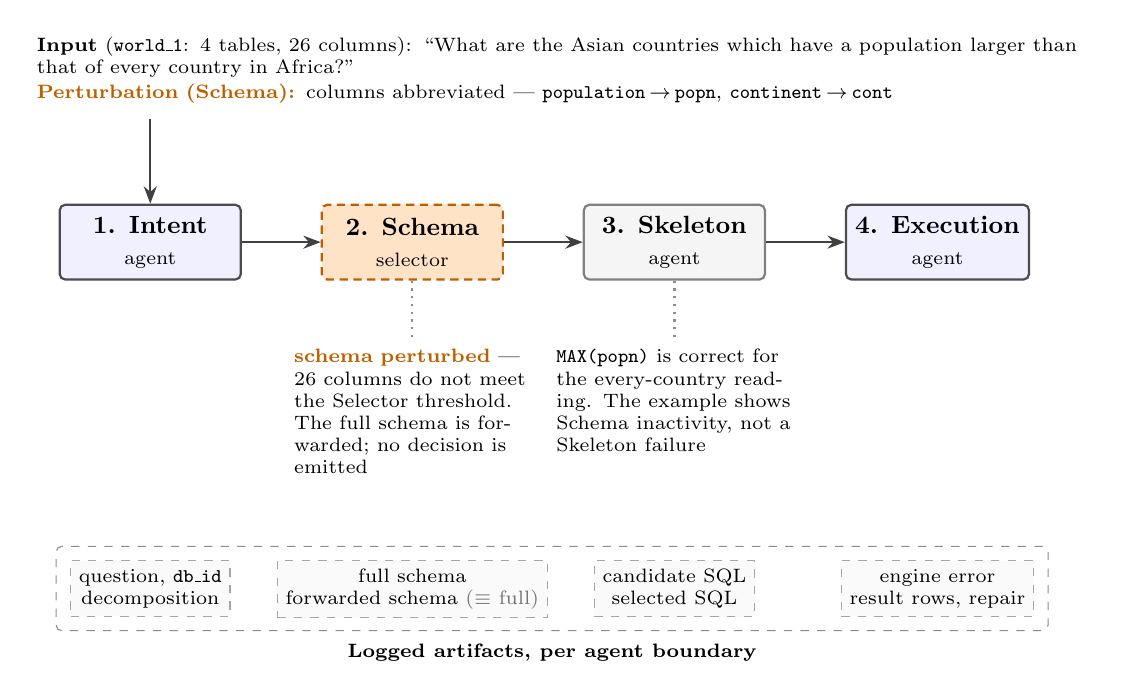
\begin{tikzpicture}[
  font=\small,
  stage/.style   = {rectangle, rounded corners=2pt, draw=black!70, thick,
                    minimum width=2.3cm, minimum height=0.95cm,
                    align=center, fill=blue!6},
  faulty/.style  = {stage, fill=orange!22, draw=orange!75!black,
                    dash pattern=on 3pt off 2pt},
  noted/.style   = {stage, fill=black!4, draw=black!50},
  logbox/.style  = {rectangle, draw=black!35, dashed, inner sep=3pt,
                    align=center, font=\scriptsize, fill=black!2},
  note/.style    = {align=left, font=\scriptsize},
  fwd/.style     = {-{Stealth[length=2.2mm]}, thick, black!75}
]
\node[stage]                            (intent)  at (0,0) {\textbf{1. Intent}\\\scriptsize agent};
\node[faulty, right=1.0cm of intent]    (schema)  {\textbf{2. Schema}\\\scriptsize selector};
\node[noted, right=1.0cm of schema]    (skeleton){\textbf{3. Skeleton}\\\scriptsize agent};
\node[stage,  right=1.0cm of skeleton]  (exec)    {\textbf{4. Execution}\\\scriptsize agent};

\draw[fwd] (intent)   -- (schema);
\draw[fwd] (schema)   -- (skeleton);
\draw[fwd] (skeleton) -- (exec);
\node[note, text width=13.6cm, anchor=south west] (q) at ([xshift=-0.4cm, yshift=1.15cm]intent.north west)
  {\textbf{Input} (\texttt{world\_1}: 4 tables, 26 columns): ``What are
   the Asian countries which have a population larger than that of every
   country in Africa?''\\[1pt]
   \textcolor{orange!75!black}{\textbf{Perturbation (Schema):}} columns
   abbreviated --- \texttt{population}\,$\to$\,\texttt{popn},
   \texttt{continent}\,$\to$\,\texttt{cont}};

\draw[fwd] ([yshift=-2pt]q.south -| intent.north) -- (intent.north);
\node[note, text width=3.0cm, anchor=north] (c1) at ([yshift=-0.75cm]schema.south)
  {\textcolor{orange!75!black}{\textbf{schema perturbed}} --- 26 columns do
   not meet the Selector threshold. The full schema is forwarded; no decision
   is emitted};

\node[note, text width=3.0cm, anchor=north] (c2) at ([yshift=-0.75cm]skeleton.south)
  {\texttt{MAX(popn)} is correct for the every-country reading. The example
   shows Schema inactivity, not a Skeleton failure};

\draw[black!45, dotted, thick] (schema.south)   -- ([yshift=1pt]c1.north);
\draw[black!45, dotted, thick] (skeleton.south) -- ([yshift=1pt]c2.north);
\node[logbox, anchor=north] (l1) at ([yshift=-3.55cm]intent.south)   {question, \texttt{db\_id}\\decomposition};
\node[logbox, anchor=north] (l2) at ([yshift=-3.55cm]schema.south)   {full schema\\forwarded schema \textcolor{black!55}{($\equiv$ full)}};
\node[logbox, anchor=north] (l3) at ([yshift=-3.55cm]skeleton.south) {candidate SQL\\selected SQL};
\node[logbox, anchor=north] (l4) at ([yshift=-3.55cm]exec.south)     {engine error\\result rows, repair};

\node[draw=black!45, dashed, rounded corners=2pt, inner sep=5pt,
      fit=(l1)(l4), label={[font=\scriptsize\bfseries, yshift=-1pt]below:%
      Logged artifacts, per agent boundary}] (matrix) {};

\end{tikzpicture}
}
\caption{The inert-stage mechanism. The fault is injected at Schema, but the
database sits below the Selector's pruning threshold, so the stage emits no
decision and the failure is attributed to Skeleton.}
\label{fig:inert}
\end{figure}

In two widely used systems a nominal stage exists, is logged faithfully, and
does nothing on most inputs of the benchmark it is run on. The Selector of MAC-SQL (Multi-Agent Collaborative framework for Text-to-SQL)~\cite{wang_mac-sql_2025} prunes only above a database-size
threshold\footnote{It prunes when $\lfloor \text{columns}/\text{tables}
\rfloor > 6$ or total columns $> 30$, so the $26$-column, $4$-table database
of Figure~\ref{fig:inert} is not pruned.}
that Spider-scale databases mostly sit below, so the full schema is forwarded
unchanged on $1{,}289$ of $1{,}700$ instances ($75.8\%$), identically under
both backbones we ran; on BIRD (BIg bench for laRge-scale Database grounded Text-to-SQL)~\cite{li_bird_2023}, whose databases are larger, the same Selector
prunes on $86.4\%$, so activity is a property of system and benchmark
together and has to be measured rather than assumed. The Decomposer of MAG-SQL (Multi-Agent Generative approach)~\cite{xie_mag-sql_2024} emits a
``decomposition'' whose sole element is the question restated verbatim on
$875$ of $1{,}534$ BIRD instances ($57.0\%$). Neither is a bug, but a
decision that was never made cannot be attributed to, and no better detector
removes that (Figure~\ref{fig:inert}).

An inert stage does not cause the failure; it removes the evidence by which
it could be localised. We therefore propose a pre-flight check-three numbers
per stage, read off logs a pipeline already produces-that tells an engineer
whether a stage can be attributed to at all: the fraction of runs on which
the stage changed its input, whether its output differs between passing and
failing runs, and the constant classifier's score on the same labels. To
exercise it we audit stage activity in two published systems and attribution
in one, instrumented at their agent boundaries, and collect $10{,}002$ runs,
re-scorable offline. Code, logs and the audit are released at
\url{https://github.com/MinhQuang0611/MAS-FailureAttribution}.

Our contributions are: (i) \emph{attributability} as three testable
conditions on a stage's artifact, and a pre-flight check that evaluates them
from existing logs; (ii) interventional evidence that inert stages bound
attributability and not accuracy, on $1{,}700$ paired runs; (iii) evidence
that Dr.\,Spider's input-perturbation labels are treatment labels, against
which attribution accuracy is not a measurement of attribution; (iv) a released
harness and $10{,}002$-run corpus, re-scorable offline, including $313$
Dr.\,Spider instances with a stage \emph{outcome} label from intervention.

The remainder of this paper is organized as follows.
Section~\ref{sec:related} reviews multi-agent Text-to-SQL, automated failure attribution and diagnostic benchmarks. Section~\ref{sec:method} describes the pipeline decomposition, the attribution procedure by backward state-differencing, the three attributability conditions and the pre-flight check. Section~\ref{sec:experiment} presents datasets, systems and comparison methods, and then reports the results: the audit of the check, attribution against chance, the label analysis, the backbone and BIRD arms, and two interventional tests (forcing the inactive stage and repairing the labelled stage), followed by a discussion of limitations. Section~\ref{sec:conclusion} concludes.

\section{Related Work}
\label{sec:related}


\subsection{Multi-agent Text-to-SQL and Stage-targeted Repair}
DIN-SQL (Decomposed In-context learning with self-correction) showed that decomposing generation into schema linking, classification
and self-correction gains roughly ten points~\cite{pourreza_din-sql_2023};
MAC-SQL~\cite{wang_mac-sql_2025} formalises a Selector-Decomposer-Refiner
triple, MAG-SQL~\cite{xie_mag-sql_2024} adds targets-conditions
decomposition and soft schema linking, CHESS (Contextual Harnessing for Efficient SQL Synthesis)~\cite{talaei_chess_2024} scales the same decomposition to large
schemas, and later systems add planning and repair agents or joint
reinforcement-learning
training~\cite{chaturvedi_sqlofthought_2025,yang_mars-sql_2025}. Error
analyses attribute over $70\%$ of parsing errors to schema linking and
joins~\cite{zhu_scot2s_2025}, catalogue error
types~\cite{shen_icl_errors_2026}, and motivate stage-targeted repair. We treat MAC-SQL and MAG-SQL as objects of
study: not how accurately they translate, but whether their stage boundaries
are visible enough to attribute failures to.

\subsection{Automated Failure Attribution}

Who\&When annotates the responsible agent and decisive step of each
trace~\cite{zhang2025which}, and FAMAS (Failure Attribution for Multi-Agent Systems)~\cite{ge_famas_2025} conditions on agent and action
activation patterns across repeated executions, so
activity-sensitive diagnosis is not new. Neither asks whether a stage that
ran also \emph{changed} its input (semantic inertness), nor what a label is
when it comes from input perturbation. Ours is a specific audit of
observability and label interpretation; it does not invalidate benchmarks
whose labels come from other procedures. MAST (Multi-Agent System failure Taxonomy) was built from $1{,}600$ human-annotated traces (Cohen's $\kappa = 0.88$)~\cite{cemri_mast_2025}, an
independent ground truth. AgenTracer~\cite{zhang_agentracer_2025} and
Aegis~\cite{kong_aegis_2025} inject faults into an agent's output, so the
injected stage is by construction the one whose artifact changed; Dr.\,Spider
perturbs the input, which only guarantees that a stage was stressed. RAFFLES (Reasoning-based Attribution of Faults for LLM Systems)~\cite{zhu_raffles_2025} replaces the
single-pass judge with iterative reasoning, FAMAS
borrows spectrum-based fault localisation, the classical
problem of recovering a cause from a downstream
symptom~\cite{wong_fault_localization_survey_2016,zeller_delta_debugging_2002};
a spectrum scorer can only rank actions that were executed. None of this
work checks whether a stage that ran also changed its input, so an
attribution benchmark reports one number in which detector quality and system
attributability are mixed together.

\subsection{Diagnostic Benchmarks}
Spider~\cite{yu_spider_2018} and its variants~\cite{lei_spider2_2025,gan_spider_syn_2021} reveal brittleness without tracing it to a stage.
Dr.\,Spider~\cite{chang_drspider_2023} fixes the stressed stage at construction time; its families are treatment labels, and no Text-to-SQL benchmark yet supplies stage \emph{outcome} labels.

\section{Methodology}
\label{sec:method}

The study asks whether a stage of a multi-agent Text-to-SQL pipeline can be
attributed to at all, and measures the answer on logged runs, in four steps:
instrumentation at agent boundaries, attribution by backward
state-differencing, an attributability audit under three conditions, and a
pre-flight check that turns the audit into three numbers per stage.

\subsection{Pipeline Decomposition and Instrumentation}

Following common practice~\cite{shen_icl_errors_2026} we model a MAS
Text-to-SQL pipeline as four stages-\emph{Intent}, \emph{Schema},
\emph{Skeleton}, \emph{Execution}-and wrap the published systems at the
boundaries between their agents, recording what each agent emitted and adding
no inference of our own: for Intent, the question and the clarified question
or decomposition; for Schema, the full schema and the subset forwarded
downstream; for Skeleton, the candidate and selected SQL; for Execution, the
engine error, result rows and any repair. Everything below is computed from
these artifacts and can be re-scored offline.

\subsection{Attribution by Backward State-Differencing}
\label{sec:attr}

The procedure under test blames a stage only when that stage's own output is
demonstrably wrong. Given a log entry and gold SQL $q^\ast$, it applies four rules in order: (i) if the schema
the Selector forwarded omits a column required by $q^\ast$, return
\textsc{Schema}; (ii) if the execution log carries a database engine error, return
\textsc{Execution}; (iii) if the Intent stage emitted a decomposition $D$ and
the content words of the question overlap those of $D$ by less than half,
return \textsc{Intent};
(iv) otherwise return \textsc{Skeleton}. The schema rule comes first because
its evidence alone is independent of the generated SQL. We call this
procedure \textsc{Attr}.

Rule (i) reads columns, not tables: MAC-SQL's Selector emits a per-table
verdict (a column list, \texttt{keep\_all}, or \texttt{drop\_all}) over every
table, so a missing-gold-table test is empty by construction; we reconstruct
what reached the Decomposer and blame Schema when a column $q^\ast$ needs did
not survive.

\subsection{Attributability: Three Conditions}
\label{sec:conditions}

Let $R$ be the logged runs, $y(r)\in\{\mathrm{pass},\mathrm{fail}\}$ the
outcome of run $r$, and for stage $s$ let $u_s(r)$ be its input and
$a_s(r)\in\mathcal{A}_s\cup\{\bot\}$ the artifact it emits ($\bot$: nothing
emitted). A detector \emph{keyed on} a property $\phi:\mathcal{A}_s\to\Phi$
is any $d=g\circ\phi$ with $g:\Phi\to\{0,1\}$ deciding whether to blame $s$;
rule (i) of \textsc{Attr} is one such $d$. Attribution to $s$ can succeed
only if three conditions hold:
\begin{align}
\text{(A1) Present:}\quad & \pi_s \;=\; \Pr_r\bigl[a_s(r)\neq\bot\bigr] \;>\; 0,
\label{eq:a1}\\
\text{(A2) Decides:}\quad & \alpha_s \;=\; \Pr_r\bigl[a_s(r)\neq u_s(r)\;\big|\;
a_s(r)\neq\bot\bigr] \;>\; 0, \label{eq:a2}\\
\text{(A3) Separable:}\quad & \delta_s(\phi) \;=\;
d_{\mathrm{TV}}\bigl(P^{\mathrm{fail}}_{\phi},\,P^{\mathrm{pass}}_{\phi}\bigr)
\;>\; 0, \label{eq:a3}
\end{align}
where $R_s^{+}=\{r: a_s(r)\neq u_s(r)\}$ is the set of active runs,
$P^{y}_{\phi}=P[\phi(a_s)\mid y,\,R_s^{+}]$ is the distribution of the keyed
property on active runs with outcome $y$, and $d_{\mathrm{TV}}$ is
total-variation distance. (A2) fails when the stage
merely restates its input: on $R\setminus R_s^{+}$ every $d$ reads the input,
not a decision of $s$, so the ceiling is zero for every detector of that form;
both of our inert stages fail here, not at (A1). For a structured artifact
$a_s = u_s$ is set equality; for a free-text one we take it to be verbatim
restatement of the input, so a paraphrase counts as active and is judged at
(A3), not here. (A3) is the strongest and is
detector-relative: for any $d=g\circ\phi$ on $R_s^{+}$, the data-processing
inequality gives
\begin{equation}
\Pr[d{=}1\mid\mathrm{fail}]-\Pr[d{=}1\mid\mathrm{pass}] \;\le\; \delta_s(\phi),
\label{eq:bound}
\end{equation}
so if $\delta_s(\phi)=0$ no detector keyed on $\phi$ separates passes
from failures, whatever $g$ is. The bound is only as wide as the property
tested: an omission test (was a gold column withheld?) bounds every
omission-keyed detector, a count test only count-keyed ones, and neither
bounds attribution methods that read other evidence.

These are coverage conditions: a statement never executed cannot be ranked by
any spectrum-based scorer~\cite{wong_fault_localization_survey_2016}. A fourth
condition sits outside the pipeline: the labels must name the stage that
failed (Section~\ref{sec:labels}). Given (A1)-(A3) we report, per stage,
present, keyable (the artifact exhibits the property the detector keys on),
fires and correct: \texttt{keyable}$=0$ is artifact-degenerate,
\texttt{fires}$=0$ with \texttt{keyable}$>0$ is our bug, and only
\texttt{correct}$=0$ with \texttt{fires}$>0$ is evidence about attribution.

\subsection{The Pre-flight Check}
\label{sec:check}

Table~\ref{box:check} turns (A1)-(A3) into a check that costs no
inference, partitioned by activity since an aggregate of an inert and an
active regime describes neither.

\begin{table}[htbp]
\centering
\fbox{\begin{minipage}{0.95\textwidth}\footnotesize
\textbf{Attributability pre-flight check.} For
each stage $s$ with artifact $a_s$, over logged runs with pass/fail outcomes:
\begin{enumerate}[leftmargin=1.4em,topsep=1pt,itemsep=0pt]
\item \textbf{Activity} ($\hat\alpha_s$, Eq.~\ref{eq:a2}). Fraction of runs on
which $a_s$ differs from $s$'s input. If $\approx 0$, stop: $s$ is
unattributable by any detector; otherwise run steps 2-3 on $R_s^{+}$ and
report both regimes.
\item \textbf{Separability} ($\delta_s(\phi)$, Eq.~\ref{eq:a3}). On $R_s^{+}$,
Fisher-test $H_0\colon \delta_s(\phi)=0$ for the property $\phi$ a detector
would key on. If $H_0$ cannot be rejected, stop: no separation is detectable at this $n$,
so by Eq.~\ref{eq:bound} no detector keyed on $\phi$ can be expected to
separate passes from failures (name $\phi$; the bound extends no further).
\item \textbf{Chance.} Report any attribution accuracy alongside the constant
classifier's score and $\kappa$ on the same labels, partitioned by activity.
\end{enumerate}
Only if all three pass is a stage-targeted detector or repair worth
funding; passing shows the artifact separates, not that the stage caused the
failure.
\end{minipage}}
\caption{The attributability pre-flight check, computable from existing logs.}
\label{box:check}
\end{table}



\section{Experiment}
\label{sec:experiment}


\subsection{Datasets and Systems}
\label{sec:setup}

We instrument MAC-SQL~\cite{wang_mac-sql_2025} and
MAG-SQL~\cite{xie_mag-sql_2024} at pinned upstream commits, wrapping each
published agent without modifying its logic.
Dr.\,Spider~\cite{chang_drspider_2023} supplies construction-time stage ground
truth: $100$ instances per family at seed $42$, $1{,}700$ over $17$ families in
three groups-NLQ ($9$ families; question rewritten, stresses Intent), DB
($3$; database perturbed, conventionally read as stressing Schema) and SQL
($5$; query structure varied, stresses Skeleton). The DB families are two that rename
schema elements (\texttt{schema\_synonym}, \texttt{schema\_abbreviation})
and one, \texttt{DBcontent\_equivalence}, rewrites cell values and touches
no schema element. BIRD~\cite{li_bird_2023} supplies no stage ground truth; its
$1{,}534$ dev instances test stage activity and artifact separability, which
need no injected fault. Queries run against local SQLite and the metric is
Execution Accuracy (EX)~\cite{yu_spider_2018}. Backbones are gpt-5.6-luna (a
closed, unversioned API model, accessed 26 Aug-18 Sep 2026) and a local
Qwen2.5-14B, identical within a comparison; $10{,}002$ runs in total
(MAC-SQL on Dr.\,Spider under both backbones plus a forced-Selector arm;
MAC-SQL, MAC-SQL without its Selector, and MAG-SQL on BIRD under
gpt-5.6-luna). Each cell is a single sweep (temperature $0.1$ for
Qwen2.5-14B, $1.0$ for gpt-5.6-luna, the only one it accepts). Re-running $410$
failing instances unchanged flips $37$ ($9.0\%$) to correct (the control arm
of the repair test below); this recovery rate among previously failed
instances is a rough guide to run-to-run variation, not a general accuracy
noise floor, and we do not read EX contrasts of that size as differences.
Four measurement errors of our own (comparator, API account, SQL extraction,
a harness bug that emptied $1{,}003$ MAG-SQL schema artifacts) were
corrected; superseded logs are excluded from every denominator and released.

\subsection{Comparison Methods and Metrics}
\label{sec:comparison}\label{sec:metrics}

\textsc{Attr} (Section~\ref{sec:attr}) is compared against a constant
classifier that always returns the most frequent stage label, and probed by
Selector arms (the same instances re-run with the pruning threshold
overridden, or with the stage removed) and interventional repair (the labelled
stage replaced by its gold value, against a control re-run unchanged).
Metrics are EX; stage recall; Cohen's $\kappa$; observed over expected correct
under a random assignment with the same marginals ($\times$ chance); and
activity and separability as in Table~\ref{box:check}.

\subsection{Results Analysis}
\label{sec:results}

\subsubsection{Stage Activity and Attribution Accuracy}

A stage \emph{acted} when it emitted a decision differing from passing its
input through. On Dr.\,Spider MAC-SQL's Selector prunes on $411$ of $1{,}700$
instances ($24.2\%$) under both backbones; MAG-SQL's Decomposer is inert on
$57.0\%$ of BIRD instances. MAC-SQL's own Decomposer emits a free-text trace
never a verbatim restatement, so it passes (A2) and is judged at (A3) in
Section~\ref{sec:audit}.

Under gpt-5.6-luna, $566$ of $1{,}700$ instances fail: $319$ carry the Intent
label, $91$ Schema and $156$ Skeleton. \textsc{Attr} gives stage recall
$71.2\%$, $6.6\%$ and $28.8\%$ and $278/566 = 49.1\%$ overall; all $6$ Schema
attributions are correct. Under Qwen2.5-14B ($661$ failures) almost everything
defaults to Skeleton.

\noindent\textbf{(1) Schema recall is conditional on the Selector having
acted.} Partitioning the $300$ DB-perturbed instances by whether the Selector
pruned gives $0/57$ against $6/34$ under gpt-5.6-luna and $0/61$ against
$16/38$ under Qwen2.5-14B. The zero survives a
change of backbone while the active half moves by a factor of $2.4$. The partition is
confounded with database size, but against the result: the pruned instances
are the harder ones (EX $54.1\%$ against $74.8\%$, Fisher
$p = 0.001$; $48.6\%$ against $73.0\%$, $p = 2{\times}10^{-4}$), yet they
hold every correct schema attribution ($p = 0.002$ and $2{\times}10^{-8}$).
These fall mostly on the wrong family: one of the six and three of the
sixteen are on the two schema-renaming families; the rest are
\texttt{DBcontent\_equivalence} instances, which touch no schema element.

\noindent\textbf{(2) Execution recall is undefined, not zero:} Dr.\,Spider
injects no execution faults, and the Refiner leaves only \textbf{one} engine
rejection among $566$ gpt-5.6-luna failures ($6$ of $661$ under Qwen2.5-14B).
\noindent\textbf{(3) Every label row shares one distribution:} each splits
between \textsc{Intent} and \textsc{Skeleton} as $71{:}29$, $67{:}33$ and
$68{:}32$ ($\chi^2 = 0.83$, $p = 0.66$): the detector reproduces the label
prior.

\subsubsection{The Instrument Audit}
\label{sec:audit}

The audit runs the four-number chain (present, keyable, fires, correct) over
both Dr.\,Spider cells. Every artifact is present; our first, table-level
Schema test reported \texttt{keyable}$=0$ in every cell and would have entered
the paper as a fact about MAC-SQL.

For Intent the keyable column coincides with the detector's firing
condition, and step 2 retires it in both cells: $67.7\%$ of failures
against $66.0\%$ of passes under gpt-5.6-luna (Fisher $p = 0.51$), $2.7\%$
against $7.7\%$ under Qwen2.5-14B ($p = 9{\times}10^{-6}$, the wrong
direction): the property tracks the backbone's verbosity, not
misunderstanding. The rule fires $381$ times and is right $227$ times under
gpt-5.6-luna ($1.06\times$ chance) and $17/17$ under Qwen2.5-14B. Skeleton,
the default, is $100\%$ on both sides by construction (at chance). The Schema artifact does separate, weakly: a gold
column is withheld in $1.1\%$ of the $566$ gpt-5.6-luna failures against
$0.0\%$ of the $1{,}134$ passes, and in $2.4\%$ against $0.9\%$ under
Qwen2.5-14B. Precision is perfect ($6/6$, $16/16$) but recall is capped in single digits;
every correct attribution lies on the $74$ pruned instances.

\subsubsection{Attribution Against Chance}
\label{sec:chance}

Dr.\,Spider's families are unbalanced: $9$ of $17$ are NLQ, so $319$ of the
$566$ gpt-5.6-luna failures carry the Intent label, and a detector that
always answered \textsc{Intent} would score $56.4\%$ against \textsc{Attr}'s
$49.1\%$ ($33.0\%$ under Qwen2.5-14B). The constant classifier wins in both
cells, and $\kappa$ is $0.056$ and $0.063$: no agreement beyond chance, so the
$49.1\%$ is an artifact of label imbalance (whether \emph{any} detector could
do better is Section~\ref{sec:labels}). Only one stage survives the
correction, and it is the one with the lowest recall: Schema runs $6.2$ and
$6.7\times$ above chance (one-sided binomial, $p = 4{\times}10^{-4}$ and
$2{\times}10^{-9}$), while Intent and Skeleton sit at
$1.0$-$1.1\times$, except Intent under Qwen2.5-14B ($1.77\times$): without a
chance baseline, recall inverts which stage is working.

\subsubsection{Label Validity}
\label{sec:labels}

One explanation for the missing skill is that the labels do not identify the
failing stage: an instance is called a schema failure because the database
was perturbed, not because the schema stage failed. If the label $L$ is independent of the failure signature
$S$, any detector $D = f(S)$ has accuracy $\sum_i p_i q_i \le \max_i p_i$,
the constant classifier's score (exact for detectors keyed on $S$,
indicative for \textsc{Attr}).

We compare each failing prediction against its gold query on two axes
independent of any attribution rule: the real column names referenced (wrong
columns: a linking fault) and the query shape-join, group by, having, order
by, aggregate (wrong shape: a construction fault). If the labels named the
failing stage, Schema-labelled failures would be dominated by column errors
and Skeleton-labelled ones by shape errors. Under gpt-5.6-luna the three label rows show
wrong columns on $33/38/31\%$ and wrong shape on $13/11/11\%$ of failures
(Intent/Schema/Skeleton; $n = 319/91/156$). A label-signature association
is not detectable ($\chi^2 = 6.22$, $\mathrm{df} = 6$, $p = 0.40$, Cram\'er's
$V = 0.07$) and small under Qwen2.5-14B ($\chi^2 = 14.92$, $p = 0.021$,
$V = 0.11$); the repair test below checks this directly.

\subsubsection{Backbone Change and BIRD}
\label{sec:bird}

A prediction fixed in advance: the schema ceiling should be stable across
backbones, since the threshold reads the database, not the model. It holds:
inert-Selector schema recall is $0$ under both backbones, on $118$ failures,
while intent recall spans $4.6$-$71.2\%$ and active-schema recall
$17.6$-$42.1\%$: what architecture bounds stays at zero, what the model
bounds moves.

A second prediction, also fixed in advance: BIRD's databases exceed the
threshold, so the Selector must act and schema attributability should be
non-zero. The antecedent holds ($1{,}325$ of $1{,}534$ pruned, $86.4\%$);
the consequent does not. The schema detector fires on $0$ of $611$ BIRD
failures: the Selector withholds a gold column in $0.0\%$ of failures and
$0.0\%$ of passes. Removing the Selector moves EX from $60.2\%$ to
$58.9\%$ ($53$ flips against $34$, McNemar $p = 0.053$; borderline, from a
single sweep): the stage acts, separates nothing, and changes little: activity is
necessary, not sufficient. MAG-SQL on the same
instances is more degenerate: Decomposer inert on $57.0\%$, intent artifact
keyable on $0.0\%$ of $605$ failures.

\subsubsection{Falsification Tests}
\label{sec:falsify}

\paragraph{An interventional test of inertness.}
\label{sec:forced}
Finding (1) contrasts different databases; on the same instances we force
the Selector to prune everywhere (all $1{,}700$ instances under
Qwen2.5-14B, the DB group under gpt-5.6-luna), predicting that schema recall
on formerly inert instances rises from $0$ while EX shifts little. No EX
change is detectable in any cell ($61.1\%$ to $61.6\%$ over all $1{,}700$ under
Qwen2.5-14B, $69.7\%$ to $68.0\%$ on the DB group under gpt-5.6-luna;
McNemar $p \ge 0.3$): inertness removes the
evidence, not, as far as we can tell, the answer. Under Qwen2.5-14B recall on inert DB failures rises
from $0/61$ to $10/65$ ($p = 0.001$); its forced Selector withholds gold
columns on $28.2\%$ of failures against $10.7\%$ of passes
($p = 3{\times}10^{-4}$), so once it acts its artifact separates. Under gpt-5.6-luna the forced Selector
withholds a gold column on $2$ of $61$ inert failures and no passes: as on
BIRD, activity is restored, attributability is not. Nor does separability
become causation: the gold schema repairs $11$ of the $103$ Qwen2.5-14B
forced-arm DB failures against $7$ for a re-run ($p = 0.46$).

\paragraph{An interventional test of the labels.}
\label{sec:counterfactual}
The interventional version of Section~\ref{sec:labels} repairs one stage
with its gold value and asks whether the failure survives. Under
gpt-5.6-luna we seed MAC-SQL's Selector through its own
\texttt{use\_gold\_schema} interface on all $91$ DB-perturbed failures (gold
tables marked \texttt{keep\_all}, only they described), hand the Decomposer
the pre-perturbation question on $313$ NLQ-perturbed failures (six of $319$
have no matching original), and re-run all $410$ failures unchanged as a
control. The original question
repairs $146$ of $313$ ($46.6\%$) against $28$ of $319$ ($8.8\%$;
$p = 6{\times}10^{-28}$), so the design has power where the label is right.
The gold schema repairs $5$ of $91$ against $9$ of $91$ in the control
(Fisher $p = 0.41$), and the split is no more favourable. On the $34$ pruned
instances, restoring the dropped columns repairs one failure and re-running
five; on the $57$ inert ones the intervention only removes non-gold tables
($4$ against $4$), so it says nothing about the label; on
\texttt{DBcontent\_equivalence}, which touches no schema element, $2$
against $7$. The informative comparison is the two renaming families,
$3/46$ against $2/46$, and at that size the arm cannot exclude repair rates
below roughly $30\%$ (Section~\ref{sec:limitations}). By the same standard our own
positive result is a treatment label, not a demonstrated cause. On the NLQ arm, \textsc{Attr} returns Intent on $65.8\%$ of the $146$
failures the original question repairs and $74.9\%$ of the $167$ it does not
($p = 0.08$): its $71.2\%$ recall is the label prior.

\subsection{Discussion and Limitations}
\label{sec:limitations}

``Inert'' is not a euphemism for ``badly built'': MAC-SQL's threshold is
cost control and MAG-SQL's Decomposer rightly declines to split a simple
question. This is an
audit of observability and label interpretation, not a claim that benchmarks
with other labelling procedures are invalid, and (A3) bounds only detectors
keyed on the property tested. Activity is also not responsibility: a stage
that should have resolved an ambiguity but skipped it is inert yet at fault,
and a superficial paraphrase counts as active without adding information, so
(A2) must be read against the stage's intended role. We did not test whether
the audit separates correct pass-through, incorrect skipping and incorrect
transformation, nor evaluate it with an attribution method stronger than
\textsc{Attr}. Every recall figure is MAC-SQL's
(CHESS~\cite{talaei_chess_2024} is BIRD-only;
MARS-SQL~\cite{yang_mars-sql_2025} needs self-hosted checkpoints on a graphics processing unit). Passing the audit is not a certificate: Schema passed it and still named
no cause. The repair arms are small: at $n = 23$ per renaming family they
have power only against repair rates above roughly $30\%$, and a
nonsignificant test means no detectable difference, not equivalence. Finally,
the label-validity test uses regular expressions, the label intervention ran under one
backbone, each cell is a single sweep, and gpt-5.6-luna is a closed,
unversioned API, so the Qwen2.5-14B arm carries the reproducibility.


\section{Conclusion}
\label{sec:conclusion}


Stage-level failure attribution assumes that each stage does something. We
found that this assumption often does not hold and should be checked before
attribution. In the two systems we studied, MAC-SQL's Selector passes its
input through unchanged on $75.8\%$ of the Spider-scale Dr.\,Spider
instances, and MAG-SQL's Decomposer copies the question word for word on
$57.0\%$ of the BIRD instances. When the Selector does nothing, schema recall
is $0/118$; when it prunes, recall is $17.6$-$42.1\%$. Forcing the Selector
to prune raises recall above zero but does not change accuracy, so an
inactive stage limits what can be attributed, not how well the pipeline
performs. Being active is still not enough: on BIRD the Selector prunes on
$86.4\%$ of instances but never removes a column the gold query needs.

On Dr.\,Spider, the Selector's output differs between passing and failing
runs when it prunes, but neither the failure patterns nor the gold-schema
repair (too small to rule out repair rates below $30\%$) show that the
failures started there. The benchmark labels tell us which stage was
perturbed, not which stage failed. Our four-rule detector agrees with these
labels no better than chance ($\kappa = 0.06$), and as long as benchmarks
provide only such labels, accuracy against them does not measure
attribution.

These results suggest two things. First, practitioners can run the
pre-flight check on the logs they already have to see whether a stage can
be diagnosed; if it cannot, there is little point in building a better
detector or a repair aimed at that stage. Second, benchmark designers can
obtain outcome labels through intervention: giving the Decomposer the
original question fixes $46.6\%$ of NLQ-perturbed failures, against $8.8\%$
for a plain re-run, and we release the $313$ instances labelled this way.
In future work we plan to audit more systems, such as CHESS on BIRD, use
larger repair sets, and repeat the label intervention with more backbones.



\bibliographystyle{splncs04}
\bibliography{failureAttribution_cr}

\end{document}
